\subsection{Компилятор} \label{sub111}

Компилятор~--- это программа, которая  принимает текст, написанный на~одном языке~--- \textit{исходном}, и~транслирует (переводит) его в~эквивалентный текст на~другом языке~--- \textit{целевом}. Одна из~важных ролей компилятора состоит в~сообщении об~ошибках в~исходной программе, обнаруженных в~процессе трансляции\cite{Aho2003}.

Процесс компиляции можно разделить на~две большие части. Первая часть~--- \textit{анализ} (выполняется несколькими анализаторами) разбивает исходную программу на~составные части и~накладывает на~них грамматическую структуру. Затем эта структура используется для промежуточного представления программы. В~процессе анализа пользователю сообщается об~ошибках, собирается информация об~исходной программе и~сохраняется в~\textit{таблицу символов}. Таблица символов~--- структуры данных, которые используются компилятором для хранения информации о~конструкциях исходной программы. Информация накапливается инкрементально в~фазе анализа компилятора и~используется фазой синтеза для генерации целевого кода.

Вторая часть~--- \textit{синтез} (выполняется генератором кода), строит требуемую целевую программу на~основе промежуточного представления и~информации из~таблицы символов.

Если рассмотреть процесс компиляции более детально, то~можно увидеть, что он~представляет собой последовательность фаз каждая из~которых преобразует одно представление программы в~другое:

\begin{itemize}
\item{\textit{Лексический анализ} или \textit{сканирование}. Лексический анализатор читает поток символов, составляющих исходную программу, группирует их в~значащие последовательности (лексемы), формирует для каждой лексемы специальные структуры данных, называемые токенами и~передает их синтаксическому анализатору.}	
\item{\textit{Синтаксический анализ} или \textit{разбор}. Синтаксический анализатор использует информацию из предыдущей фазы и~на её основе строит синтаксическое дерево, в~котором каждый внутренний узел представляет операцию, а~дочерние узлы~--- аргументы этой операции.}	
\item{\textit{Семантический анализ}. Эта фаза компиляции использует синтаксическое дерево и~информацию из таблицы символов для проверки исходной программы на семантическую согласованность с~определением языка. Важной частью семантического анализа является проверка и~приведение типов.}	
\item{\textit{Генерация промежуточного кода.} На этой фазе компилятор генерирует низкоуровневое промежуточное представление кода исходной программы, которое можно рассматривать как программу для абстрактной вычислительной машины.}	
\item{\textit{Машинно-независимая оптимизация кода.} Фаза машинно-независимой оптимизации кода пытается улучшить промежуточный код.}	
\item{\textit{Генерация кода.} В качестве исходных данных генератор кода получает промежуточное представление исходной программы и~отображает его в~целевой язык, как правило в~ассемблерный код.}
\item{\textit{Машинно-зависимая оптимизация кода.} Фаза машинно-зависимой оптимизации кода улучшает код целевой машины, учитывая особенности архитектуры процессора.}		
\end{itemize}

Фазы компиляции, которым соответствуют одноименные исполнители, представлены на рис.~\ref{img:compiler-structure}.

\begin{figure}[ht]
	\centering
	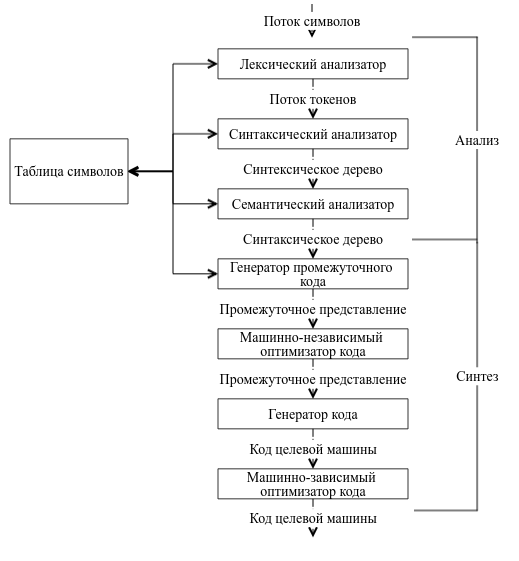
\includegraphics [scale=0.9] {compiler-structure}
	\caption{Схема взаимодействия фаз компилятора}
	\label{img:compiler-structure}
\end{figure}

Процесс анализа компиляции разделен на~лексический, синтаксический и~семантический анализ по~ряду причин: 

\begin{enumerate} 
	\item{Упрощение разработки. Отделение лексического анализа от~синтаксического позволяет упростить как минимум одну из~фаз анализа. Например, включить в синтаксический анализатор работу с~комментариями и~пробельными символами существенно сложнее, чем удалить их~лексическим анализатором.}
	\item{Увеличение эффективности компилятора. Отдельный лексический анализатор позволяет применять более специализированные методики, предназначенные исключительно для решения лексических задач.}
	\item{Увеличение переносимости компилятора. Особенности устройств ввода могут быть ограниченны лексическим анализатором.}
	\item{Разделение зон ответственности. Ошибки типизации будут выявлены на~стадии семантического анализа, что позволит сформулировать сообщение об~ошибках типизации в~более полной мере.}
\end{enumerate}
